\chapter{Building our 3D Sketch}

Every time I design a cable and pulley system, I struggle through the same
questions. How does a 3D sketch work? Do I need a 3D sketch? Should I make the cables first or the pulleys first?

Sometimes I decide ``I don't actually need to CAD the cables.'' Time saved by
not cadding the cables is dwarfed by the time spent modifying hardware later, say
when the cables run directly through another part.

\section{Our Notation}

Throughout this tutorial, we'll use the following notation:

\begin{itemize}
\item{} \emph{Italics} is used to denote sketch and feature names, such as \emph{Line 1} and
  \emph{Pulley 1}. While SolidWorks may apply a name like ``Line1@Sketch2'', we'll ignore those names and rename them ourselves.
\item{} \kode{Green code} is used to notate SolidWorks features that you should click, such as \relation{Extrude}, \relation{Circle}, and \relation{Concentric}.
\item{} \texttt{Typewriter text} is used to denote keystrokes, such as \texttt{Tab}
  and \texttt{R}. Here, \texttt{R} refers to pressing the \texttt{R} key alone,
  not in a capitalized form.

\texttt{Shift+R} refers to ``Hold \texttt{Shift} and press \texttt{R}''.
\item{} Constraints will be described as below, which reads ``Add a
    \relation{Coincident}
  relation between \emph{Line 1} and \emph{Line 2}.''
\end{itemize}

\begin{center}
\begin{tabular}{ccc}
  \hline
  \relation{Coincident} & \emph{Line 1} & \emph{Line 2} \\
  \hline
\end{tabular}
\end{center}

\begin{itemize}
  \item{} Removing constraints will be described as below, which reads ``Remove
    the existing \relation{Coincident} relation between \emph{Line 1} and
    \emph{Line 2}.''
\end{itemize}

\begin{center}
\begin{tabular}{ccc}
  \hline
  \xrelation{Coincident} & \emph{\sout{Line 1}} & \emph{\sout{Line 2}} \\
  \hline
\end{tabular}
\end{center}

\subsection{Modifying the Pace}

\label{sec:modifying_the_pace}
This tutorial is designed for those with basic SolidWorks skills. I only explain
the concepts relevant to 3D sketches and the relevant features. For those who
find the pace too slow, each section is summarized with a \textbf{Section Recap}.
These steps, along with the images and a few mental leaps, should keep the pace
appropriate.

\subsection{Overview}

\label{sec:overview}

In this tutorial, we'll make a pulley/cable system, utilizing SolidWorks 3D
sketching capabilities. We will start by sketching a system of planar pulleys (Section~\ref{sec:planar-pulleys}), turning our
sketches into a multi-body part (Section~\ref{sec:making_solid_bodies}). We will
then progressively make the system more complicated, moving the system off the
cardinal plane (Section~\ref{sec:non_orthogonal_pulleys}) and making the cables non-tangential to the pulleys (Section~\ref{sec:non-tangential-pulleys}).

\section{Planar Pulleys and Cables}

\label{sec:planar-pulleys}

Our first goal is to make a two-pulley system where both pulleys and the entire
cable lie in the same plane. A preview of our completed system is shown in
Figure~\ref{fig:completed-planar}. The 3D sketch used to create this system, and
the primary sketch we'll be working with for the rest of this tutorial, is shown in
Figure~\ref{fig:completed-planar-3d-sketch}.

\begin{figure}[H]
\begin{center}
  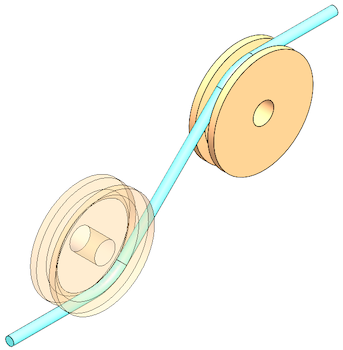
\includegraphics[height=2.25in]{images/figures/completed-planar.png}
\end{center}
\caption{Completed cable-pulley system with all components in one plane. One pulley is
transparent for clarity. \label{fig:completed-planar}}

\end{figure}

\begin{figure}[H]
\begin{center}
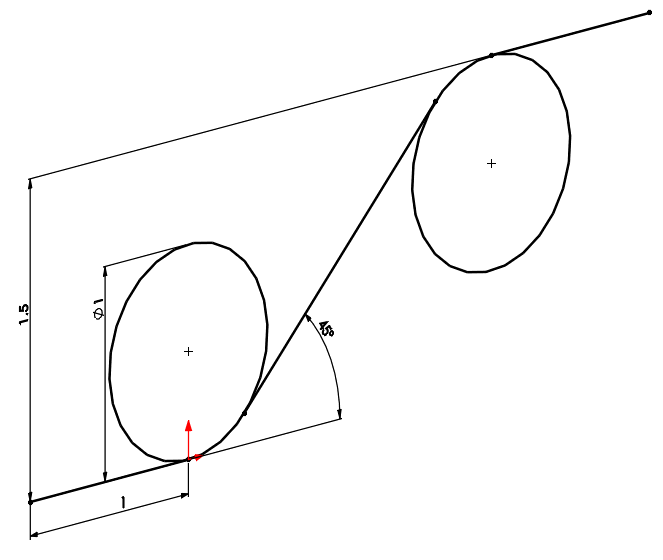
\includegraphics[height=3.5in]{images/figures/completed-planar-3d-sketch.png}
\end{center}
\caption{Completed 3D sketch. This sketch is fully on the right plane, but we're using
a 3D sketch because we will later move entities off the right plane.
\label{fig:completed-planar-3d-sketch}}
\end{figure}

Make a new part with ``Inch, Pound, Second (IPS)'' units (though for our purposes,
``Inch, Stone, Fortnight'' units would also get the job done.) \relation{Save}
this file. I used the name "Cable Pulley System - Rev 0", so that if I later
revise it, I don't have to get too creative in renaming the file. This
will be our working part for the remainder of the tutorial.

\subsection{Making Line 1}

\label{sec:making_line_1}

First, switch to an isometric view. For the rest of this tutorial, an Isometric
view will orient my coorinate system as follows. Don't fret if yours doesn't
match, you can simply adapt.

\begin{figure}[H]
\begin{center}
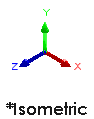
\includegraphics{images/figures/Coordinate-System.png}
\end{center}
\end{figure}

Create a new \relation{3D Sketch} by selecting the dropdown arrow beside
\relation{Sketch}.

\begin{figure}[H]
\begin{center}
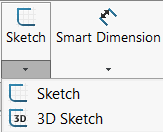
\includegraphics{images/symbols/3D-Sketch-Button.png}
\end{center}
\end{figure}

Unlike 2D sketches, 3D sketches are not associated with a sketch plane. Their entities
can exist anywhere in space. Select the \relation{Line} tool. Note that the cursor displays the plane you are drawing
on. In our case, use \texttt{Tab} to
switch to the \emph{Z-X Plane}. Add a line along
the positive Z-Axis, as shown in Figure~\ref{fig:making-line-1}.

\begin{figure}[H]
\begin{center}
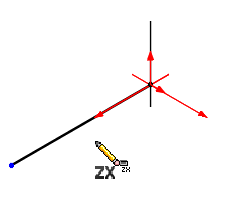
\includegraphics{images/figures/Making-Line-1.png}
\end{center}
\caption{Make \emph{Line 1} along the positive Z axis. Use the \texttt{Tab} key to switch the drawing plane within the 3D sketch. \label{fig:making-line-1}}
\end{figure}

If your line turns black after clicking, it is automatically constrained
\\ \relation{Along-Z}. The endpoint (still blue) is not yet constrained. Yellow relations that appear when adding entities will be automatically added after
clicking, whereas white relations that appear near your cursor are not added. If your relation was not added, add that relation now.

Finally, \relation{Dimension} \emph{Line 1} to 1'' long. The sketch is now fully constrained.

The labels we'll use for this and the other sketch entities are shown in
Figure~\ref{fig:labeled-sketch}.

\begin{figure}[H]
\begin{center}
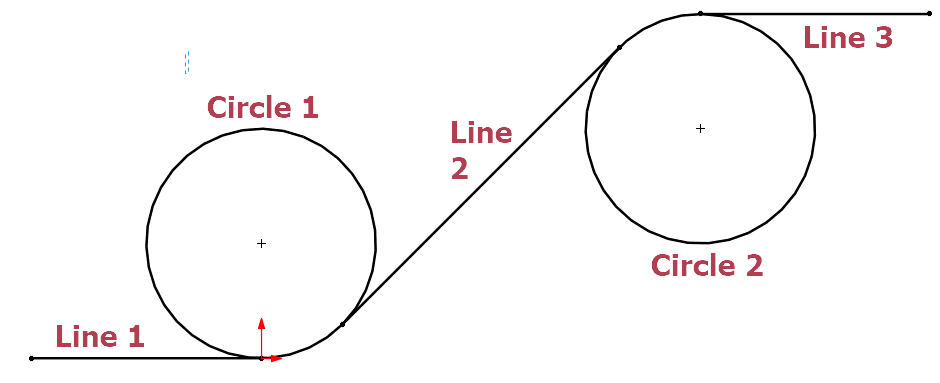
\includegraphics[height=2.5in]{images/figures/labeled-sketch.png}
\end{center}
\caption{Though SolidWorks gives each sketch entity a name, we'll use these
names instead. \label{fig:labeled-sketch}}
\end{figure}

\subsubsection{Section Recap}

\begin{enumerate}
\item{} Select an isometric view.
\item{} Create a \relation{3D Sketch}.
\item{} Select the \relation{Line} tool.
\item{} Use the \texttt{Tab} key to change which plane you are sketching on.
\item{} Sketch a \relation{Line} (\emph{Line 1}) along the positive Z axis.
\item{} If not already done, add an \relation{Along-Z} relation to \emph{Line 1}.
\item{} Dimension \emph{Line 1} to 1'' long.
\end{enumerate}

\subsection{Making Circle 1}

\label{sec:making-circle-1}
Still working in the 3D Sketch but now on the Y-Z Plane, add a \relation{Circle}, which we'll
call \emph{Circle 1}, whose
perimeter intersects the origin. A \relation{Coincident} relation should
automatically be
added. Dimension \emph{Circle 1} to 1'' in diameter.

\begin{figure}[H]
\begin{center}
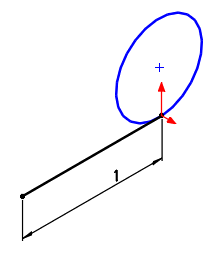
\includegraphics{images/figures/Making-Circle-1.png}
\end{center}
\caption{Make \emph{Circle 1} coincident with the origin and on the Y-Z Plane.
\label{making-circle-1}}

\end{figure}

Next, add the \relation{Tangent} relation between \emph{Circle 1} and \emph{Line
1}. I'd add it in the following way:

\begin{enumerate}
\item{} Select \emph{Circle 1}
\item{} Hold the \texttt{Ctrl} key.
\item{} Select \emph{Line 1}
\item{} Release the \texttt{Ctrl} key.
\item{} Press \texttt{Alt+A} to create the relation.

We can see which letter to use by which letter is underlined in the "Add
Relations" sidebar.
\end{enumerate}

Note that even though we drew \emph{Circle 1} on the Y-Z plane, it is not constrained
to that plane and we can drag it around. Add an
\relation{On-Plane} relation with the Right Plane.

Circle 1 is now fully constrained.

\subsubsection{Section Recap}

\begin{enumerate}
\item{} Make a \relation{Circle} (\emph{Circle 1}) on the Y-Z Plane.
\item{} Make that circle \relation{Coincident} and \relation{Tangent} with
  \emph{Line 1} at the \emph{Origin}.
\item{} Constrain \emph{Circle 1} to \relation{On-Plane} with the \emph{Right
  Plane}.
\end{enumerate}

\subsection{Making Circle 2}

Create another \kode{Circle} and constrain it as follows:

\begin{center}
\begin{tabular}{rcc}
  \hline
  \relation{On-Plane} & \emph{Circle 1} & \emph{Right Plane} \\
  \relation{Equal} & \emph{Circle 1} & \emph{Circle 2} \\
  \hline
\end{tabular}
\end{center}

A surprising SolidWorks feature, entities in 3-D sketches can be manipulated
with the \relation{Triad}, found by right-clicking on the entity. Use the
\kode{Triad} to position \emph{Circle 2} as shown in Figure~\ref{fig:labeled-sketch}. Using the \kode{Triad}
here is academic. As sketches get more complicated, it can be a lifesaver.

\subsubsection{Section Recap}

\begin{enumerate}
\item{} Make a \relation{Circle} (\emph{Circle 2}) on the X-Z Plane.
\item{} Constrain \emph{Circle 2} \relation{On-Plane} with the \emph{Right Plane}.
\item{} Constrain \emph{Circle 2} \relation{On-Plane} to \emph{Circle 1}
\item{} Position \emph{Circle 2} with the \relation{Triad}, just for practice.
\end{enumerate}

\subsection{Making Line 2 and Line 3}

Add a \relation{Line} (\emph{Line 2}) connecting \emph{Circle 1} and \emph{Circle 2}. Constrain
it as follows, confirming that the tangent relations snap to the correct side of
\emph{Circles 1 \& 2}, as in Figure~\ref{fig:completed-planar-3d-sketch}.

\begin{center}
\begin{tabular}{rcc}
  \hline
  \relation{Tangent} &
  \emph{Line 2} & \emph{Circle 1} \\
  \relation{Tangent} &
  \emph{Line 2} & \emph{Circle 2} \\
  \hline
\end{tabular}
\end{center}

Add a \kode{Line} (\emph{Line 3}) with one endpoint coincident to \emph{Circle 2} and extending
parallel to \emph{Line 1}. Constrain it as follows:

\begin{center}
\begin{tabular}{rcc}
  \hline
  \relation{Along-Z}
  \emph{Line 3} & \emph{Circle 1} \\
  \relation{Equal}
  \emph{Line 3} & \emph{Line 1} \\
  \relation{Tangent}
  \emph{Line 3} & \emph{Circle 2} \\
  \hline
\end{tabular}
\end{center}

\subsection{Constraining the 3D Sketch}

Moving \emph{Circle 2} with the \kode{Triad} shows us that we are missing two
constraints, as in Figure~\ref{fig:unconstrained-entities}.
First, nothing defines the angle between \emph{Line 1} and \emph{Line 2}. Second, nothing
defines the length of \emph{Line 2}. There are many options that fill our need, but
let's try to choose constraints that convey physical meaning and design intent.


\begin{figure}[H]
\begin{center}
  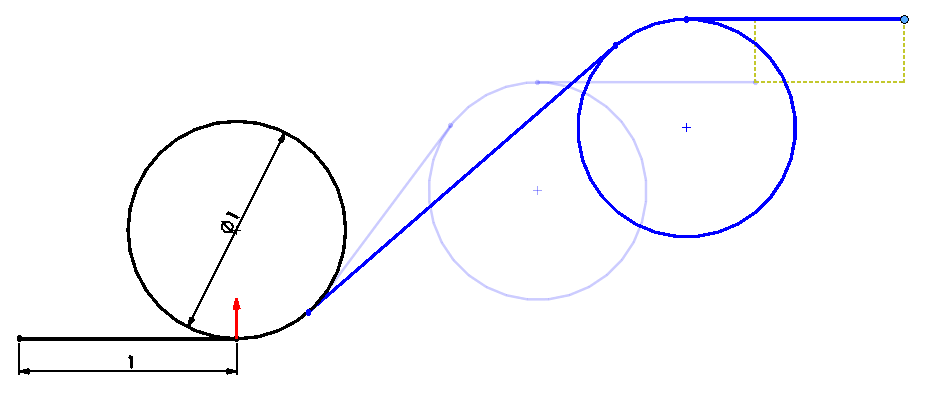
\includegraphics[height=2in]{images/figures/unconstrained-entities.png}
\end{center}
\caption{Missing dimensions mean we can change both the height of \emph{Line 3}
  and the angle of \emph{Line 2}.
\label{fig:unconstrained-entities}}
\end{figure}

Among the many constraint choices in pulley-cable systems, I'll often choose to
define the angle that the cable wraps around the pulley. This is meaningful
because it defines the load experienced by the pulley. Dimension the minor angle between \emph{Line 1}
and \emph{Line 2} to 45\textdegree.

\begin{figure}[H]
\begin{center}
  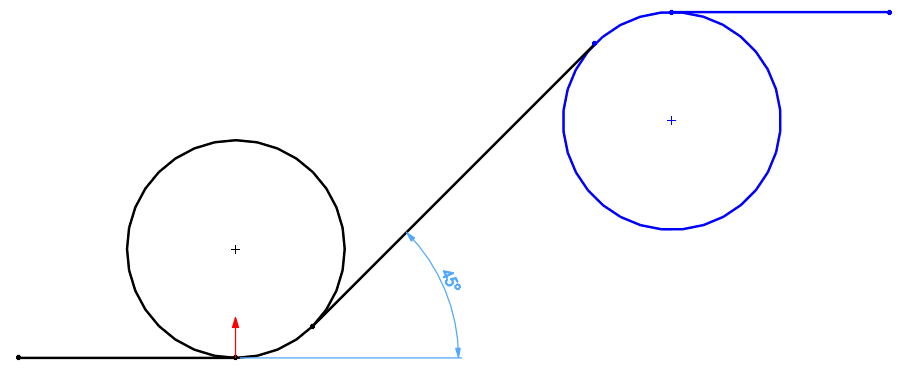
\includegraphics[height=2in]{images/figures/cable-wrap-dimension.png}
\end{center}
\end{figure}

Second, let's define the parallel distance between \emph{Line 1} and \emph{Line 3}.
Presumably, we're using pulleys to relocate the cable from where it wants to be (i.e.
straight between its endpoints) to where we want it (e.g. an S-bend). This
parallel distance defines how large an S-bend we impart on the cable. Add a
parallel distance dimension of 1.5'' between \emph{Line 1} and \emph{Line 3}.

\begin{figure}[H]
\begin{center}
  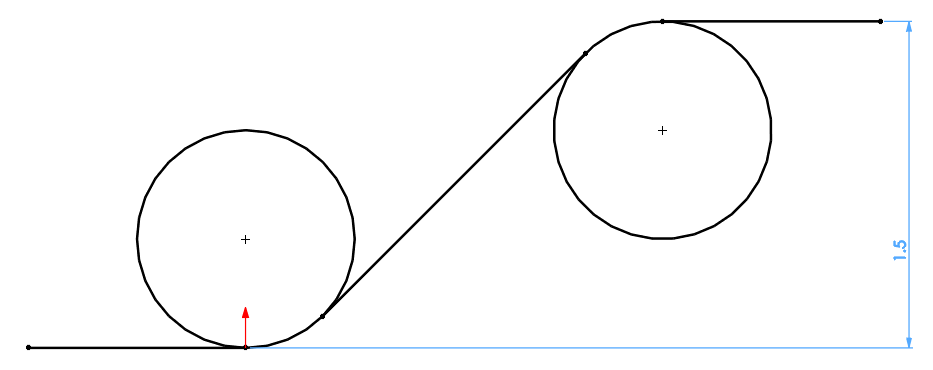
\includegraphics[height=2in]{images/figures/s-bend-dimension.png}
\end{center}
\end{figure}

Congratulations! Our 3D sketch is now fully constrained. Celebrate by closing
the sketch\cadsymbol{close-sketch} and saving \cadsymbol{Save}.

\subsubsection{Section Recap}

\begin{enumerate}
\item{} Dimension the angle between \emph{Line 1} and \emph{Line 2} to 45\textdegree.
\item{} Dimension the parallel distance between \emph{Line 1} and \emph{Line 3} to 1.5''.
\item{} Exit the sketch.
\item{} Save early and save often.
\end{enumerate}
